% !TEX root = MAIN.tex

\section{DaMAT}

\begin{figure}[h]
  \centering
	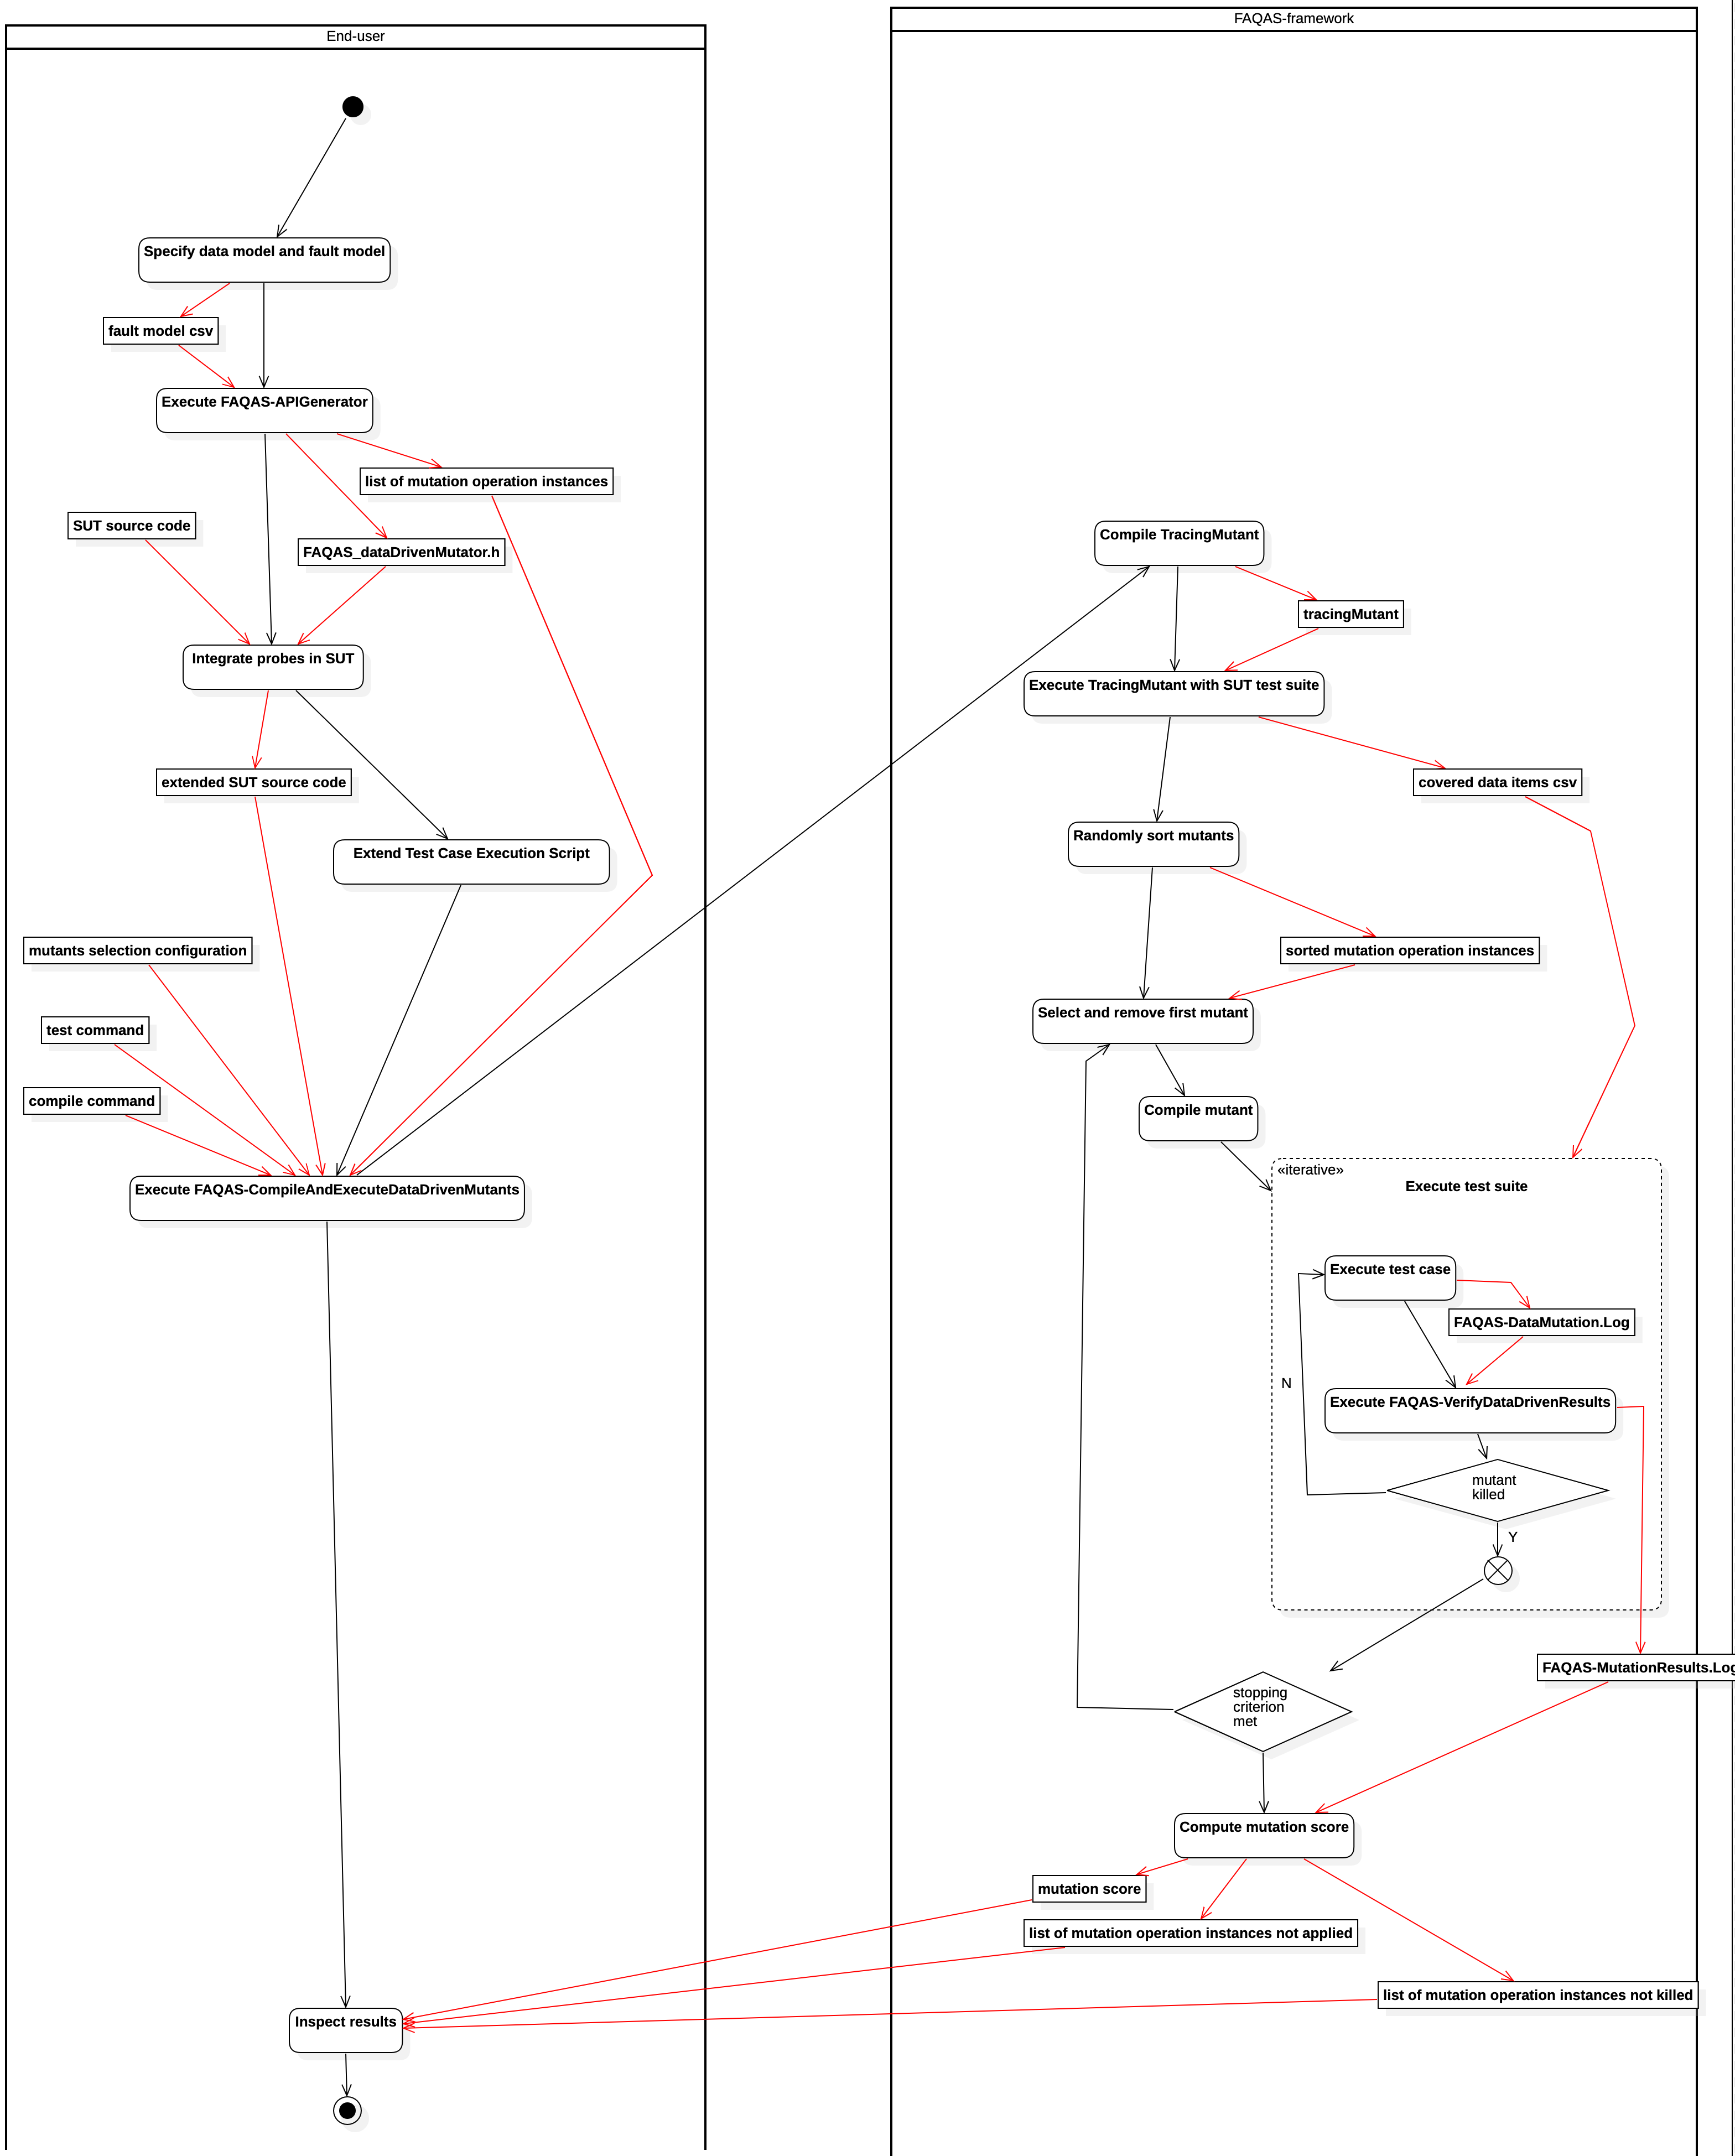
\includegraphics[width=\textwidth]{images/png/Activity1!DataDrivenTestSuiteEvaluation_3.png}
      \caption{Overview of the data-driven mutation testing process to evaluate test suite effectiveness.}
      \label{fig:process:dataDriven:evaluation}
\end{figure}

The data-driven mutation testing component shall implement the process for the evaluation of test suite effectiveness that is drafted in Figure~\ref{fig:process:dataDriven:evaluation}. Figure~\ref{fig:process:dataDriven:evaluation} relies on UML activity diagram notation. In Figure~\ref{fig:process:dataDriven:evaluation} the execution of specific software artefacts by the end-user is made explicit. Also, we use black arrows to draw control-flow, red arrows for data-flow. 

The activity \emph{Specify data model and fault model} in Figure~\ref{fig:process:dataDriven:evaluation} indicates that the engineer should prepare a csv file specifying the fault model and the data model for the SUT according to D2.

The activity \emph{Execute FAQAS-APIGenerator} in Figure~\ref{fig:process:dataDriven:evaluation} concerns the execution of the program \emph{Execute FAQAS-APIGenerator}.

The program \emph{FAQAS-APIGenerator} takes as input the \emph{fault model csv} and generates the file \emph{FAQAS\_dataDrivenMutator.h} and a csv file containing the \emph{list of mutation operation instances} derived from the fault model.

File \emph{FAQAS\_dataDrivenMutator.h} contains the FAQAS mutation testing API (i.e., the predefined functions to perform data mutation for buffers) and the fault model represented as a data structure. Details are provided in D2.

The activity \emph{Integrate probes in SUT} in Figure~\ref{fig:process:dataDriven:evaluation} indicates that the engineer should manually modify the source code of the SUT to integrate mutation probes into it. Examples are provided in \emph{Listing 2.3}, \emph{Listing 3.1}, and \emph{Appendix A - Section 1.1} of D2. 

The activity \emph{Extend Test Case Execution Script} in Figure~\ref{fig:process:dataDriven:evaluation} indicates that the engineer is expected to manually modify the scripts used to execute test cases so that they include an invocation to \emph{FAQAS-VerifyDataDrivenResults} after the execution of every single test case. 

The activity \emph{Execute FAQAS-CompileAndExecuteDataDrivenMutants} in Figure~\ref{fig:process:dataDriven:evaluation} concerns the execution of the program \emph{Execute FAQAS-CompileAndExecuteDataDrivenMutants}.

The program \emph{Execute FAQAS-CompileAndExecuteDataDrivenMutants} receives as inputs the command to compile the SUT, the command to execute the test suite, the path to the extended SUT source code, and the mutants selection configuration. It automatically executes a number of activities required to compute the mutation score: \emph{Compile TracingMutant}, \emph{Execute TracingMutant with SUT test suite}, \emph{Randomly sort mutants}, \emph{Select and remove first mutant}, \emph{Compile mutant}, \emph{Execute test suite},  \emph{Compute mutation score}.

The program \emph{FAQAS-CompileAndExecuteDataDrivenMutants} implements the four mutants selection strategies: \emph{all mutants} (i.e., all the mutants are tested), \emph{proportional uniform sampling} (i.e., a subset of the mutants is tested selected based on a percentage), \emph{uniform fixed-size sampling} (i.e., a subset of the mutants is tested selected based on a fixed number), and \emph{uniform FSCI sampling} (i.e., a subset of the mutants is tested, they are selected according to the FSCI criterion).

The \emph{mutants selection configuration} indicates the mutants selection strategy and a configuration value that specifies the number of mutants to consider; the value may indicate the percentage of mutants to sample (for \emph{proportional uniform sampling}), the number of mutants to sample (for \emph{uniform fixed-size sampling}), or the size of the confidence interval (for \emph{uniform FSCI sampling}).

The activity \emph{Compile TracingMutant} indicates that the system compiles a version of the SUT that traces the data items (targeted by mutation) that are covered by each test case (see D2, Figure 2.9, line 5).

The activity \emph{Execute TracingMutant with SUT test suite} indicates that the system executes the SUT test suite. Since the test suite is executed with the TracingMutant it leads to the generation of a csv files that indicates, for every test case, the data items being exercised by the test case.

The activity \emph{Randomly sort mutants} indicates that  \emph{FAQAS-CompileAndExecuteDataDrivenMutants} generates a randomly sorted list of mutation operation instances. This list is derived from the \emph{list of mutation operation instances}.

The activity \emph{Select and remove first mutant} indicates that  \emph{FAQAS-CompileAndExecuteMutants} selects the first item in the \emph{sorted mutation operation instances} and removes it from the list.

The activity \emph{Compile mutant} indicates that the system compiles a version of the SUT with the selected mutation operation instance enabled.

The activity \emph{Execute test case} indicates that the test suite of the SUT executes a test case. Only the test cases exercising the data item targeted by the mutation operator are executed. Since the test case is executed against the mutated SUT, if the mutation operation is performed, then the file \emph{FAQAS-MutationResults.Log} will be created (this is a feature of the FAQAS data-driven mutation API).

File \emph{FAQAS-MutationResults.Log} contains the ID of the mutation operation instance applied.

Program \emph{FAQAS-VerifyDataDrivenResults} receives as input the ID of the test case and  the status of a test case (i.e., PASS or FAIL). It checks if a data mutation operator has been applied based on the content of \emph{FAQAS-DataMutation.Log}. It deletes \emph{FAQAS-DataMutation.Log}. It updates the content of \emph{FAQAS-MutationResults.Log}.

If program \emph{FAQAS-VerifyDataDrivenResults} determines that a mutation operation instance has been killed, then the test suite execution is terminated.

File \emph{FAQAS-MutationResults.Log} indicates, for every executed test case, the ID of the mutation operation instance applied and the mutation result (KILLED or LIVE). A test case may appear multiple times in this file, each time with a different mutation operation instance ID associated.

The execution of the test suite is repeated till a termination criterion is met. The termination criterion depends on the mutants selection strategy:
\begin{itemize}
\item \emph{all mutants}: the list \emph{sorted list of mutants} is empty
\item \emph{proportional uniform sampling}: a number of mutants matching the selected percentage has been executed
\item \emph{uniform fixed-size sampling}: a number of mutants matching the selected value has been executed
\item \emph{uniform FSCI sampling}: the confidence interval computed from \emph{mutation results csv} is smaller than the length specified by the user.
\end{itemize}

The activity \emph{Compile mutation score} concerns the computation of the mutation score based on the mutation results reported in \emph{FAQAS-MutationResults.Log}. The formula is provided in D2. As output of the computation of the mutation score the system reports also the \emph{list of mutation operation instances not killed} and the \emph{list of mutation operation instances not applied}. The \emph{list of mutation operation instances not killed} includes also the name of test cases executed for each, to facilitate the improvement of the test suite.

The end-user inspects the \emph{list of mutation operation instances not applied} to understand which data types had not been covered by the test suite. The end-user inspects the \emph{list of mutation operation instances not killed} to understand which test cases need improvement.




